% UPAR 2027 Track 1 paper, WACV 2026 author kit (the format required by the RWS workshop at WACV 2027).
\documentclass[10pt,twocolumn,letterpaper]{article}

%%%%%%%%% PAPER TYPE: \usepackage[review,algorithms]{wacv} for the anonymous review version
\usepackage{wacv}

%
% --- inline annotations
%
\newcommand{\red}[1]{{\color{red}#1}}
\newcommand{\todo}[1]{{\color{red}#1}}
\newcommand{\TODO}[1]{\textbf{\color{red}[TODO: #1]}}
% --- disable by uncommenting  
% \renewcommand{\TODO}[1]{}
% \renewcommand{\todo}[1]{#1}


\usepackage{booktabs}
\usepackage{multirow}
\usepackage{amsmath}
\usepackage{graphicx}
\graphicspath{{figs/}}

\definecolor{wacvblue}{rgb}{0.21,0.49,0.74}
\usepackage[pagebackref,breaklinks,colorlinks,allcolors=wacvblue]{hyperref}
\usepackage[capitalize]{cleveref}

\def\wacvPaperID{*****}
\def\confName{WACV}
\def\confYear{2027}
\newcommand{\pts}{\,pts}

\title{Source Gains Do Not Transfer:\\Designing Pedestrian Attribute Recognition for Unseen Cameras}

\author{Anonymous Authors\\
UPAR Challenge 2027, Track 1}

\begin{document}
\maketitle

%=====================================================================
\begin{abstract}
A pedestrian attribute recognizer is usually improved by tuning it on validation data from its training cameras. We show that, for a camera the model has never seen, such improvements are an unreliable guide. In leave-one-dataset-out experiments, per-attribute thresholds fitted on source validation data raise the source score by 0.55 points but lower the held-out score by 0.53. Deeper fine-tuning raises the source score of every encoder we tried, while its held-out effect changes sign between encoders and its gain does not survive on the hidden test set. We trace both effects to one cause. Parameters estimated on the source datasets absorb their cameras and labelling conventions, which are precisely what change on a new domain. Two design rules follow. Diversity should come from pretraining, not from fitting, so we pair a self-supervised DINOv3 and an image-text CLIP encoder, and we find that a partner's held-out thresholded accuracy, rather than its ranking quality, predicts the gain of the pair. Thresholds should come from the metric, not from source labels, so we derive a one-parameter correction from balanced accuracy that recovers about 40\% of the threshold error measured by an oracle. The resulting system scores 0.7997 Challenge\_Avg on the hidden test set of UPAR 2027 Track~1.
\end{abstract}

\begin{figure*}[t]
\centering
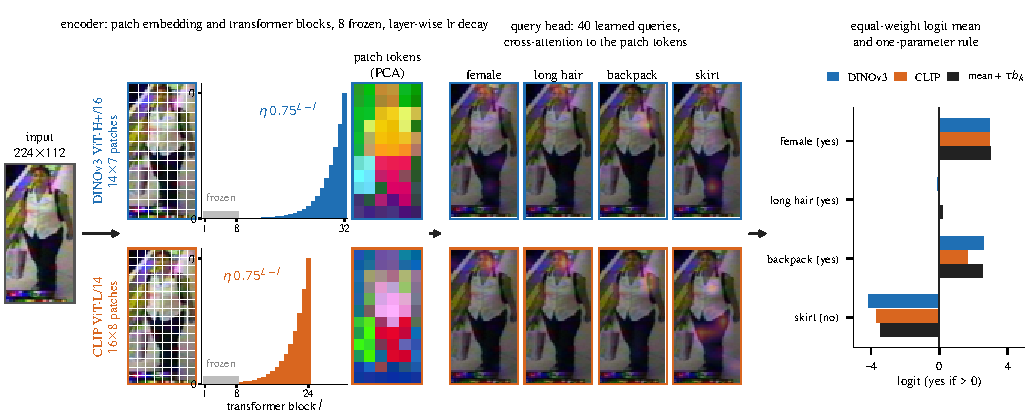
\includegraphics[width=\linewidth]{architecture.pdf}
\caption{Architecture of the system on a PETA image. Each row is one encoder: its patch grid, the learning rate of each transformer block during fine-tuning, and its patch tokens shown by their first three principal components. Each attribute query attends to the tokens, and the logits of the two encoders are averaged and shifted by the decision rule. Tokens, attention and logits come from the ViT-L members of \cref{sec:limits}, which never saw PETA during training.}
\label{fig:arch}
\end{figure*}

%=====================================================================
\section{Introduction}
\label{sec:intro}

Searching surveillance footage for ``a woman in a pink top with a backpack'' needs a pedestrian attribute recognizer that works on cameras it has never seen. The usual PAR benchmarks~\cite{peta,pa100k,market} cannot measure this, because they draw training and test images from the same cameras. The UPAR challenges~\cite{upar,upar23,upar24} were created for this purpose. They train on several public datasets and test on a domain from which no training image comes.

The standard way to improve such a recognizer is to tune it on validation data from the training cameras. Thresholds are fitted per attribute, the depth of fine-tuning is chosen, and ensemble members are weighted, each by the score they produce on that data. This practice assumes that what improves the source will improve the target. On a new domain we find that the assumption fails. When we hold out one of the three training datasets, per-attribute thresholds fitted on the source raise the source score and lower the held-out score by almost the same amount. Deeper fine-tuning raises the source score of every encoder, yet its held-out effect changes sign between encoders, and on the hidden test set it loses.

The reason is that the source datasets differ from the target in exactly the properties these parameters learn. Cameras differ in resolution and color rendering, and annotators differ in how they name colors, sleeve lengths and accessories. A threshold fitted on PETA learns that PETA marks two colors for one garment in 12\% of cases, a convention the other datasets almost never follow. The more a parameter is fitted to the source, the more of these properties it absorbs. Measured with an oracle, the resulting threshold error alone costs about three points of the challenge score on a held-out dataset, on top of a four-point loss in ranking quality.

This diagnosis gives two design rules, and our system follows them. First, diversity should come from pretraining, which is fixed, rather than from fitting. We pair a self-supervised DINOv3 encoder~\cite{dinov3} with an image-text CLIP encoder~\cite{clip}, fine-tune both only in their upper blocks and average them with fixed equal weights. \Cref{fig:arch} shows the resulting system on an image from a dataset that neither encoder saw during training. Second, thresholds should come from the metric rather than from source labels. We derive a correction with a single coefficient from the balanced-accuracy half of the metric, whose optimum does not depend on the label distribution of the target domain. Our contributions are findings about what transfers to an unseen camera:
\begin{itemize}
\item For three common tuning choices, gains measured on the source domains do not predict gains on held-out domains, and the hidden test agrees (\cref{sec:transfer}).
\item When encoders are combined under a thresholded metric, the partner's own held-out accuracy predicts the gain of the pair, while its ranking quality does not. Distilling the pair into one encoder removes the gain (\cref{sec:pairing,sec:combining}).
\item A threshold correction derived from the metric recovers part of the threshold error, and an oracle bounds the part that no rule estimated from the source can recover (\cref{sec:rule}).
\end{itemize}


%=====================================================================
\section{Related Work}
\label{sec:related}

\paragraph{Pedestrian attribute recognition.} DeepMAR~\cite{deepmar} framed PAR as multi-label classification with a loss weighted by attribute frequency, a weighting still widely used. Later methods added modules that localize attributes or model their relations, but Jia~\etal~\cite{rethinkpar} showed that many of these gains disappear under a stricter split, a first sign that in-domain improvements may not reflect generalization. Query-based heads~\cite{q2l,mldecoder} give each label its own query over the image tokens, and we use one as a standard component. UPAR~\cite{upar} unified four datasets into 40 attributes and made cross-domain evaluation possible.

\paragraph{Generalization with pretrained encoders.} With a strong backbone, plain empirical risk minimization matches specialized domain generalization methods~\cite{domainbed}. Kumar~\etal~\cite{lpft} showed that full fine-tuning improves in-distribution accuracy but can lower out-of-distribution accuracy because it distorts pretrained features, and weight interpolation with the pretrained model~\cite{wiseft} restores some robustness. Weight averaging of fine-tuned models~\cite{soups,diwa} improves robustness at no inference cost. These works concern the encoder. We extend the question to every source-fitted part of a PAR system, including thresholds and ensemble weights.

\paragraph{Ensembles under distribution shift.} The error of an ensemble falls with the accuracy of its members and with their disagreement~\cite{krogh}, and deep ensembles remain among the most reliable predictors under dataset shift~\cite{deepens,ovadia}. Which of the two factors matters when the members are fine-tuned foundation encoders and the metric is thresholded has, to our knowledge, not been measured.

\paragraph{Label shift and logit adjustment.} When class priors change, posteriors can be corrected by the ratio of priors~\cite{saerens,lipton}, and adding a scaled log prior to the logits optimizes balanced error~\cite{logitadj}. Our correction applies this idea to a multi-label metric and removes the shift already introduced by the DeepMAR loss weights.

%=====================================================================
\section{Setting}
\label{sec:setting}

\paragraph{Task and metric.} Each pedestrian crop has 40 binary attributes, covering age (three classes), gender, hair length (three classes), sleeve length, lower-body length and type, twelve upper-body and twelve lower-body clothing colors, and five accessories. The training data are the UPAR re-annotations of PA100k, Market1501 and PETA (\cref{tab:data}), and the hidden test set holds 29{,}248 images from a fourth domain. The challenge score Challenge\_Avg (Avg) is the harmonic mean of two quantities. The first, mA, is the balanced accuracy averaged over attributes. The second, instance F1, is the F1 score of each image's predicted attribute set, averaged over images. Both use a fixed threshold of 0.5. We report scores $\times100$ and differences in points (pts).

\begin{table}[t]
\centering\small
\setlength{\tabcolsep}{3pt}
\resizebox{\columnwidth}{!}{%
\begin{tabular}{@{}lrrl@{}}
\toprule
Dataset & Train & Val & Images \\
\midrule
PA100k~\cite{pa100k} & 79{,}001 & 9{,}986 & outdoor, about 600 cameras \\
Market1501~\cite{market,marketattr} & 10{,}000 & 16{,}458 & one campus, $128\times64$ crops \\
PETA~\cite{peta} & 8{,}668 & 6{,}963 & ten pooled sources \\
\bottomrule
\end{tabular}}
\caption{Training data of UPAR 2027 Track~1.}
\label{tab:data}
\end{table}

\paragraph{Held-out protocol.} Because the target domain is unseen, we evaluate each choice on a domain the model has not seen either. We train on the training splits of two datasets and score the validation split of the third. PETA, whose ten pooled sources make it the most varied, is the main held-out domain, and Market1501 serves as a second one for the key comparisons. For the PETA-held-out models, the validation images of Market1501 and PA100k give a source score on images not used in training. Each choice is therefore measured twice, on the source and on a held-out domain, and the comparison of the two is the central measurement of this paper. Protocol models are trained for three epochs on two datasets, and the submitted models for three epochs on the training and validation splits of all three.

\paragraph{Noise.} Four runs of CLIP ViT-L/14 with the same recipe, differing only in seed, machine or activation implementation, score between 81.13 and 81.58 on held-out PETA. Paired with the same DINOv3 model, they score between 82.17 and 82.42. We therefore treat differences below about 0.3\pts{} between single runs as unreliable.

%=====================================================================
\section{Source Gains Do Not Transfer}
\label{sec:transfer}

We start from the system of \cref{sec:design}, a pair of DINOv3 ViT-H+ and CLIP ViT-L encoders with a one-parameter threshold rule, and replace one part at a time by the alternative that standard practice would tune on the source (\cref{tab:fitting}). Each alternative is fitted or selected where the source score is measured.

The source scores move in one direction. Fitted per-attribute thresholds, deeper fine-tuning and a tuned member weight all raise them, although the gain of fitted thresholds is optimistic because it is measured on the data used for fitting. The held-out scores do not follow. Fitted thresholds lose on PETA about as much as they gain on the source. Deeper fine-tuning, which freezes four instead of eight blocks and gives the middle blocks of ViT-H+ about twenty times larger learning rates, helps DINOv3 on both held-out domains but hurts CLIP on PETA. In the pair, its held-out effect lies within the noise band, and on the hidden test set it loses (\cref{sec:test}). The member weight is the one fitted quantity that does no harm, because the weight that is best on the source is almost exactly the equal weight.

\begin{table}[t]
\centering\small
\setlength{\tabcolsep}{3pt}
\resizebox{\columnwidth}{!}{%
\begin{tabular}{@{}llccc@{}}
\toprule
Our choice & Source-tuned alternative & source & PETA & Market1501 \\
\midrule
one-parameter rule & fitted per-attribute thresholds & +0.55 & $-$0.53 & -- \\
conservative fine-tuning & deeper, DINOv3-H+ alone & +0.51 & +0.59 & +0.18 \\
conservative fine-tuning & deeper, CLIP-L alone & +0.44 & $-$0.44 & +0.03 \\
conservative fine-tuning & deeper DINOv3 in the pair & +0.21 & +0.18 & +0.07 \\
equal weights & best source weight (0.6) & +0.01 & $-$0.04 & +0.11 \\
\bottomrule
\end{tabular}}
\caption{Change in Avg when a part of the system is replaced by an alternative tuned on the source domains.}
\label{tab:fitting}
\end{table}

Two measurements on held-out PETA show why the source misleads. The first concerns ranking. The mean AUC of the pair, which does not depend on any threshold, falls from 96.71 on the source images to 92.97 on PETA, so the model orders images less correctly on the new domain. The second concerns thresholds. We fit one offset per attribute on the held-out labels themselves, an oracle that cannot be used at test time but bounds what any threshold rule could achieve. With plain thresholds at 0.5, the oracle gains 3.09\pts{} on PETA and 2.54\pts{} on Market1501. In earlier experiments on the same protocol we traced most of this gap to clothing colors, the attributes whose labelling conventions differ most between datasets. Both losses come from properties of the source that a fitted parameter absorbs, and fitting the source more closely enlarges rather than removes them. The design of the next section therefore draws its accuracy from components that are not fitted to the source.

%=====================================================================
\section{Design for an Unseen Camera}
\label{sec:design}

\subsection{System}
\label{sec:system}

\Cref{fig:arch} shows the system on a PETA image. It is assembled from standard components, chosen by the two design rules of \cref{sec:intro}.

\paragraph{Encoders.} Two foundation encoders from different pretraining families provide the diversity of the system. DINOv3 ViT-H+/16~\cite{dinov3} is trained by self-distillation on images alone, while CLIP ViT-L/14~\cite{clip} is trained to match images with captions. Both read a $224\times112$ crop. To keep their features close to pretraining, the patch embedding and the first eight transformer blocks are frozen, and the remaining blocks are trained with layer-wise learning-rate decay~\cite{beit} of 0.75 per block, which concentrates the update in the top blocks.

\paragraph{Head and loss.} A query head~\cite{q2l,mldecoder} gives each of the 40 attributes a learned query that attends to the encoder tokens with one cross-attention layer, followed by an MLP and a classifier owned by that attribute. In \cref{fig:arch} the queries settle on the regions their attributes describe, although neither encoder saw PETA during training. The loss is binary cross-entropy with label smoothing 0.05 and the DeepMAR weights~\cite{deepmar} $w_k^{+}=e^{1-\pi_k}$ and $w_k^{-}=e^{\pi_k}$, where $\pi_k$ is the training prior of attribute $k$. Datasets are sampled in proportion to $N_d^{0.5}$, and the remaining details are in \cref{app:config}.

\paragraph{Combination.} The two encoders produce one logit per attribute, which we average with fixed equal weights. Averaging logits rather than probabilities lets a confident member outweigh an uncertain one. The averaged logit then passes through the threshold correction of \cref{sec:rule}.


\subsection{Choosing the partner encoder}
\label{sec:pairing}

If accuracy is to come from pretraining, the most important choice is the second encoder. We fine-tuned ten foundation encoders with the same recipe and paired each with DINOv3 ViT-H+ (\cref{tab:encoders}). On held-out PETA, CLIP ViT-L/14 is the best partner, followed by the closely related MetaCLIP ViT-L/14~\cite{metaclip}. On the source images the order of these two is reversed, by a margin far below the noise band.

The table also shows what makes a partner good, and ranking quality alone does not. Both SigLIP2 encoders~\cite{siglip2} rank PETA about as well as CLIP, with a similar AUC, yet they form two of the four weakest pairs. Across the nine partners, the partner's own held-out Avg predicts the pair's Avg with a Spearman correlation of 0.92, whereas its AUC reaches only 0.42. The SigLIP2 encoders produce more false positives than CLIP on rare attributes such as glasses, old age and baldness, and averaging with DINOv3 does not remove them. Under a thresholded metric, a partner contributes through its decisions and not only through its ordering, so it should be chosen by its held-out accuracy. Selecting by the source score would have picked MetaCLIP, whose pair is slightly better on the source and clearly worse on PETA, another instance of the pattern of \cref{sec:transfer}.

\begin{table}[t]
\centering\small
\setlength{\tabcolsep}{2.6pt}
\resizebox{\columnwidth}{!}{%
\begin{tabular}{@{}llccccc@{}}
\toprule
& & \multicolumn{3}{c}{single encoder} & \multicolumn{2}{c}{with DINOv3-H+} \\
\cmidrule(lr){3-5}\cmidrule(l){6-7}
Encoder & Input & PETA & AUC & source & PETA & source \\
\midrule
DINOv3 ViT-H+/16~\cite{dinov3} & 224$\times$112 & 81.42 & 92.23 & 88.66 & -- & -- \\
\midrule
CLIP ViT-L/14~\cite{clip} & 224$\times$112 & 81.54 & 91.87 & 88.38 & 82.33 & 89.14 \\
MetaCLIP ViT-L/14~\cite{metaclip} & 224$\times$112 & 81.35 & 92.04 & 88.51 & 82.14 & 89.19 \\
EVA02-CLIP ViT-L/14~\cite{evaclip} & 224$\times$112 & 80.58 & 90.97 & 87.94 & 82.03 & 89.02 \\
AIMv2 ViT-L/14~\cite{aimv2} & 224$\times$112 & 80.23 & 91.40 & 87.82 & 81.90 & 88.96 \\
PE-Core ViT-L/14~\cite{pe} & 224$\times$112 & 80.71 & 91.23 & 88.06 & 81.88 & 89.02 \\
MetaCLIP2 ViT-H/14~\cite{metaclip2} & 168$\times$84 & 80.42 & 91.63 & 87.29 & 81.87 & 88.84 \\
SigLIP2 So400m/14~\cite{siglip2} & 224$\times$112 & 80.12 & 91.67 & 87.60 & 81.86 & 88.94 \\
SigLIP2 ViT-L/16~\cite{siglip2} & 256$\times$128 & 80.12 & 91.76 & 87.81 & 81.68 & 89.01 \\
DFN-CLIP ViT-L/14~\cite{dfn} & 224$\times$112 & 79.37 & 90.87 & 86.95 & 81.63 & 88.78 \\
\bottomrule
\end{tabular}}
\caption{Encoders alone and paired with DINOv3 ViT-H+ by logit averaging, with PETA held out during training.}
\label{tab:encoders}
\end{table}

\subsection{Weighting, extending or compressing the pair}
\label{sec:combining}

With the partner chosen, three alternatives to the equal-weight pair remain (\cref{tab:design}). The first weights the members. The best weight differs between domains. On PETA it is the equal weight, while on Market1501 it moves towards DINOv3, which alone is as good as any mixture there. Equal weights stay within 0.11\pts{} of the best weight on both domains, whereas relying on one encoder loses up to 0.91\pts{} on one of them. Without knowledge of the target domain, equal weights are the safe choice.

The second alternative adds a third member, and none of four candidates improves the pair, including MetaCLIP2 ViT-H/14, the largest encoder we tried. A third member mostly resembles one already present, and on a thresholded metric its false positives weigh as much as its corrections.

The third alternative compresses the pair into a single encoder of the same size. We distilled an ensemble of DINOv3 ViT-H+, CLIP ViT-L/14 and MetaCLIP2 ViT-H/14 into one DINOv3 ViT-H+ student, using soft targets~\cite{hinton} on mixed inputs for 15 epochs. The student alone is as accurate as the best single encoder of this study. Paired with CLIP, however, it gains less than the original DINOv3 model does, because it has absorbed CLIP's predictions and no longer disagrees with it. \Cref{fig:cases} shows what such disagreement contributes. In the backpack example, DINOv3 is confidently right, CLIP is wrong with less confidence, and the averaged logit follows DINOv3. The pairing gain thus depends on members trained independently, which an equal-weight ensemble preserves and a distilled student does not.

\begin{table}[t]
\centering\small
\setlength{\tabcolsep}{4pt}
\begin{tabular}{@{}lcc@{}}
\toprule
Variant & PETA & Market1501 \\
\midrule
DINOv3-H+ + CLIP-L, equal weights & 82.33 & 86.35 \\
\quad weight of DINOv3-H+ 0.4 & 82.30 & 86.23 \\
\quad weight of DINOv3-H+ 0.6 & 82.29 & 86.46 \\
\quad DINOv3-H+ alone & 81.42 & 86.46 \\
\quad CLIP-L alone & 81.54 & 85.60 \\
\midrule
+ MetaCLIP ViT-L/14 & 82.32 & -- \\
+ MetaCLIP2 ViT-H/14 & 82.27 & -- \\
+ AIMv2 ViT-L/14 & 82.16 & -- \\
+ SigLIP2 So400m/14 & 82.15 & -- \\
\midrule
distilled DINOv3-H+ student alone & 82.00 & -- \\
distilled student + CLIP-L & 82.21 & -- \\
\bottomrule
\end{tabular}
\caption{Weighting, extending and compressing the pair, with each domain held out during training.}
\label{tab:design}
\end{table}

\begin{figure*}[t]
\centering
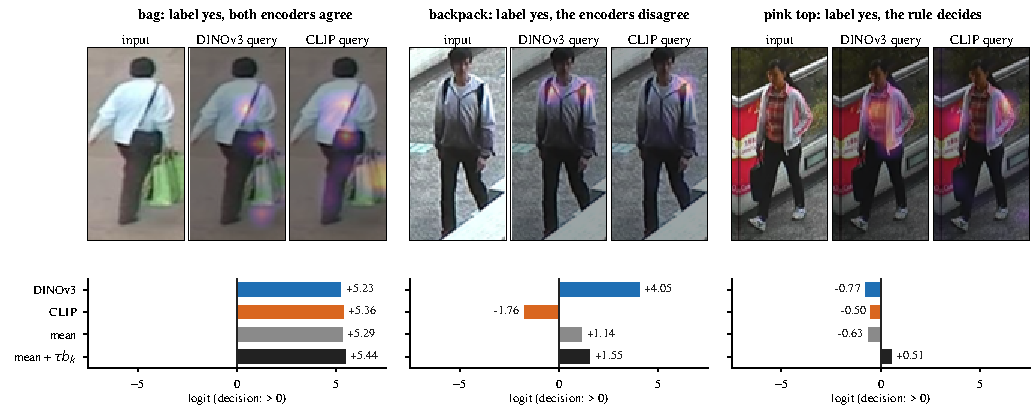
\includegraphics[width=\linewidth]{method_cases.pdf}
\caption{Three PETA cases for encoders that never saw PETA. Top: input and the attention of each encoder's query for the named attribute. Bottom: the logit of each encoder, their mean, and the mean after the decision rule.}
\label{fig:cases}
\end{figure*}

\subsection{A threshold correction from the metric}
\label{sec:rule}

\Cref{sec:transfer} showed that thresholds fitted on the source learn its conventions. They are also noisy, because many attributes have few positives. A threshold rule for an unseen domain should instead have few parameters, and its target should not depend on the label distribution of that domain.

The mA half of the metric supplies such a target. Balanced accuracy weighs positives and negatives equally, so its optimal decision is the one made under a balanced prior, whatever the true prior of the target domain is. If the model is calibrated under the training prior $\pi_k$, moving to a balanced prior adds $\log\frac{1-\pi_k}{\pi_k}$ to the logit~\cite{saerens,logitadj}. The DeepMAR weights have already moved the optimum of the training loss by $\log(w_k^{+}/w_k^{-})=1-2\pi_k$ in the same direction, so only the difference remains to be added to the averaged logit $\bar z_k$,
\begin{equation}
b_k=\log\frac{1-\pi_k}{\pi_k}-(1-2\pi_k),\qquad z_k \leftarrow \bar z_k+\tau\,b_k .
\label{eq:rule}
\end{equation}
Instance F1, the other half of the metric, prefers fewer positives for rare attributes. A single coefficient $\tau\in[0,1]$ trades the two halves off, from the decision of the weighted loss at $\tau=0$ to the mA-optimal decision at $\tau=1$. For a rare attribute such as a pink top ($\pi_k\approx0.02$), $b_k$ is large and positive, which is why the rule turns the correct but negative mean logit of the third case in \cref{fig:cases} into a positive decision. For a frequent attribute such as trousers ($\pi_k\approx0.9$), $b_k$ is negative. We use $\tau=0.42$, a value set in earlier single-model experiments on the PETA-held-out protocol, with priors from all training and validation labels. Because the derivation ignores label smoothing and assumes calibration under $\pi_k$, it fixes the form of the rule rather than the value of $\tau$.

\Cref{fig:tau} shows how much the rule recovers and how sensitive it is to its single parameter. On PETA it raises the pair by 1.24\pts{} over the plain threshold, and on Market1501 by 0.84\pts, which closes about 40\% and a third of the oracle gap of \cref{sec:transfer}. The single encoders gain by similar amounts, so the rule and the ensemble correct different parts of the error and their gains add up. All curves rise until $\tau$ reaches 0.5 to 0.65 and collapse soon after, when rare attributes are predicted far too often and instance F1 breaks down. The value $\tau=0.42$, chosen before these models existed, lies on the rising part on both domains, close to the best value and away from the collapse. The rest of the oracle gap, 1.85\pts{} on PETA and 1.70\pts{} on Market1501, is larger than every difference between encoders in \cref{tab:encoders}. It depends on the conventions of the target domain, so no rule estimated from the source can recover it.

\begin{figure}[t]
\centering
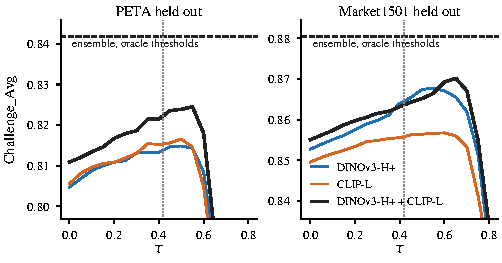
\includegraphics[width=\linewidth]{tau_rule.pdf}
\caption{Challenge\_Avg as a function of the coefficient $\tau$ on two held-out domains. The dotted line marks the submitted value and the dashed line the pair with oracle thresholds.}
\label{fig:tau}
\end{figure}

%=====================================================================
\section{Hidden-Test Results}
\label{sec:test}

The hidden test is the final check of both the protocol and the claim of \cref{sec:transfer}. \Cref{tab:test} lists our main submissions with the PETA-held-out score of each recipe. The protocol orders the first three submissions as the test does. Moving from a single distilled DINOv3 ViT-L to an ensemble of four models gains 0.63\pts{} on the test set. Replacing that ensemble by the DINOv3 ViT-H+ and CLIP ViT-L pair, which is smaller and better on the protocol, adds 0.22\pts. The protocol score of v20 uses the ten-epoch student of v13 in place of its longer-trained student. The fourth submission applies the deeper fine-tuning of \cref{tab:fitting}. Its held-out gain lies inside the noise band, and on the test set it loses 0.10\pts, the outcome \cref{sec:transfer} predicts for a change that mainly fits the source. The submitted system v21 reaches an mA of 80.61 and an instance F1 of 79.33 on the test set, with precision 75.61 and recall 84.90.

\begin{table}[t]
\centering\small
\setlength{\tabcolsep}{3pt}
\resizebox{\columnwidth}{!}{%
\begin{tabular}{@{}llcc@{}}
\toprule
& Members & PETA held out & Hidden test \\
\midrule
v13 & distilled DINOv3 ViT-L/16 student & 81.18 & 79.12 \\
v20 & student + DINOv3 ViT-L + CLIP-L + MetaCLIP2-H & 82.03 & 79.75 \\
v21 & DINOv3 ViT-H+ + CLIP ViT-L (this paper) & 82.33 & 79.97 \\
v22 & v21 with deeper DINOv3 fine-tuning & 82.51 & 79.87 \\
\bottomrule
\end{tabular}}
\caption{Submissions to UPAR 2027 Track~1 and the protocol scores of their recipes.}
\label{tab:test}
\end{table}

%=====================================================================
\section{Conclusion}
\label{sec:conclusion}

On an unseen camera, gains measured on the training cameras are an unreliable guide, because the parameters that produce them absorb the conventions of the source datasets. Designing against this cause leads to a simple system. Two encoders from different pretraining families are fine-tuned only in their upper blocks and averaged with equal weights, the partner is chosen by its held-out accuracy, and one coefficient derived from the metric sets all thresholds. The largest remaining error lies in the labelling conventions of the target domain, which no component fitted on the source can learn, and closing it would require at least some knowledge of how the target is labelled.

\paragraph{Limitations.}\label{sec:limits} Most comparisons rest on one held-out dataset and one training run per configuration, and the noise estimate comes from one encoder. \Cref{fig:arch,fig:cases} use the ViT-L members of an earlier pair of the same two families, trained with the same recipe, because the held-out version of the submitted ViT-H+ model was not kept. The threshold correction assumes priors estimated from representative training data.

\paragraph{Broader impact.} Attribute recognition on surveillance video, including age and gender, can support tracking of individuals. We report technical findings only and do not release models trained on surveillance data.

{\small
\bibliographystyle{ieeenat_fullname}
\bibliography{refs}
}

%=====================================================================
\clearpage
\appendix
\section{Training configuration}
\label{app:config}

Both encoders use the same recipe. The optimizer is AdamW with learning rate $5\cdot10^{-5}$ at the last block, layer decay 0.75, a head learning rate ten times larger, weight decay 0.05 and batch size 64. The schedule is cosine with half an epoch of warm-up and lasts three epochs. Training uses stochastic depth 0.1, bf16 mixed precision and an exponential moving average of the weights with decay 0.9995, which is the model used at test time. The query head has one layer, eight attention heads, an MLP ratio of two and dropout 0.1. Augmentation consists of random down-scaling to simulate low-resolution crops, horizontal flip, edge padding of ten pixels followed by a random crop, brightness, contrast and saturation jitter without hue change, Gaussian blur and random erasing. Priors $\pi_k$ are clipped to $[10^{-3},1-10^{-3}]$, and cells that a dataset does not annotate are masked in the loss. The two submitted members are trained on the training and validation splits of all three datasets. At test time both read the same crop resized to $224\times112$, and the pair processes the 29{,}248 test images in about four minutes on one NVIDIA A10 GPU.

\end{document}
